\documentclass[12pt,a4paper]{article}
\usepackage{amsmath,amscd,amsbsy,amssymb,latexsym,url,bm,amsthm}
\usepackage{epsfig,graphicx,subfigure}
\usepackage{enumitem,balance}
\usepackage{wrapfig}
\usepackage{mathrsfs,euscript}
\usepackage[usenames]{xcolor}
\usepackage{hyperref}
\usepackage[vlined,ruled,linesnumbered]{algorithm2e}
\usepackage{array}
\hypersetup{colorlinks=true,linkcolor=black}

\newtheorem{theorem}{Theorem}
\newtheorem{lemma}[theorem]{Lemma}
\newtheorem{proposition}[theorem]{Proposition}
\newtheorem{corollary}[theorem]{Corollary}
\newtheorem{exercise}{Exercise}
\newtheorem*{solution}{Solution}
\newtheorem{definition}{Definition}
\theoremstyle{definition}

\renewcommand{\thefootnote}{\fnsymbol{footnote}}

\newcommand{\postscript}[2]
 {\setlength{\epsfxsize}{#2\hsize}
  \centerline{\epsfbox{#1}}}

\renewcommand{\baselinestretch}{1.0}

\setlength{\oddsidemargin}{-0.365in}
\setlength{\evensidemargin}{-0.365in}
\setlength{\topmargin}{-0.3in}
\setlength{\headheight}{0in}
\setlength{\headsep}{0in}
\setlength{\textheight}{10.1in}
\setlength{\textwidth}{7in}
\makeatletter \renewenvironment{proof}[1][Proof] {\par\pushQED{\qed}\normalfont\topsep6\p@\@plus6\p@\relax\trivlist\item[\hskip\labelsep\bfseries#1\@addpunct{.}]\ignorespaces}{\popQED\endtrivlist\@endpefalse} \makeatother
\makeatletter
\renewenvironment{solution}[1][Solution] {\par\pushQED{\qed}\normalfont\topsep6\p@\@plus6\p@\relax\trivlist\item[\hskip\labelsep\bfseries#1\@addpunct{.}]\ignorespaces}{\popQED\endtrivlist\@endpefalse} \makeatother

\usepackage{tikz}
\usepackage{tcolorbox}
\tcbuselibrary{skins}
\tcbsubskin{mycross}{empty}{frame code={%
    \draw[line width=1pt] (frame.south west)--(frame.north east);
    \draw[line width=1pt] (frame.north west)--(frame.south east);},
    skin first=mycross,skin middle=mycross,skin last=mycross 
}
\usepackage{float}


\begin{document}
\noindent

%========================================================================
\noindent\framebox[\linewidth]{\shortstack[c]{
\Large{\textbf{Lab09-Network Flow}}\vspace{1mm}\\
CS214-Algorithm and Complexity, Xiaofeng Gao \& Lei Wang, Spring 2021.}}
\begin{center}
\footnotesize{\color{red}$*$ If there is any problem, please contact TA Yihao Xie. }

\footnotesize{\color{blue}$*$ Name: Log Creative  \quad Student ID:  \quad Email: logcreative-lzl@sjtu.edu.cn}
\end{center}

\begin{enumerate}
    \item  Consider there is a network consists $n$ computers. For some pairs of computers, a wire $i$ exists in the pair, which means these two computers can communicate with each other. When a signal passes through the wires, the noise in the signal will be amplified. If you know the magnification rate of noise $m_{i,j}$ of each wire (which must be greater than 1). Design an algorithm to find the route for each other computer to send signals to the computer $v$ with the minimum total magnification rate of noise and analyze the time complexity.
    
	\begin{solution}
		% Similar to Dijkstra Algorithm
		To solve the problem, the model has to be first simpilified.
		\begin{lemma}[No loop]\label{lem:nl}
			There is no loop on the optimized route.
		\end{lemma}

		\begin{figure}[h]
			\centering
			\begin{tikzpicture}[node distance=10pt]
\tikzstyle{blackdot} = [circle,fill, scale=0.3];
\node [blackdot] (v1) at (-1.5,0.5) {};
\node [below of=v1] {$A$};
\node [blackdot] (v2) at (1,0.5) {};
\node [below of=v2] {$B$};
\draw[->,line width=2pt,blue!50] (-3.5,0.5) -- (v1) -- (v2) -- (3,0.5);
\node [blackdot] (v3) at (-1.5,2.5) {};
\draw[->,line width=1pt,red!50]  plot[smooth, tension=.99] coordinates {(v1) (-0.5,1.5) (v3) (-2.5,1.5) (-1.5,0.5)};
\node[red!50] at (1,2) {$\prod_{L\backslash p}m_{ij}>1$};
\end{tikzpicture}
			\caption{A loop.}
			\label{fig:lp}
		\end{figure}

		\textbf{Proof of Lemma \ref{lem:nl}.} \textbf{Prove by contradiction.} Suppose there is a loop on the optimized route. Because the maginification on each wire $m_{ij}>1$, shown in Figure \ref{fig:lp}, if their is a loop $L$ between node $A$ to node $B$, a better way is to just choose the path $p$ directly from $A$ to $B$,
		\begin{equation*}
			\prod_{m_{ij}\not\in L} m_{ij} \prod_{m_{ij}\in L} > \prod_{m_{ij}\not\in L} m_{ij} \prod_{m_{ij}\in p} m_{ij} \cdot 1
		\end{equation*}
		This will make the following lemma available.
		\hfil \qed \vspace{\parskip}

		\begin{lemma}[Computer to computer]\label{lem:c2c}
			It is equivilent to consider the minimized maginification path between computer and the other computer.
		\end{lemma}
		\begin{figure}
			\centering
			\begin{tikzpicture}[node distance=10pt]
\tikzstyle{blackdot} = [circle,fill, scale=0.3];

\node [blackdot] (v1) at (-1.5,1) {};
\node [blackdot] (v3) at (1,1) {};
\node [blackdot] (v2) at (0,-0.5) {};
\node[above of=v1] {$A$};
\node[above of=v3] {$C$};
\node[below of=v2] {$B$};
\draw[bend left]  (v1) edge node[right] {$m_{AB}$} (v2);
\draw[bend right,line width=1pt]  (v1) edge node[left] {$m_{AB}^\prime$} (v2);
\draw  (v2) edge node[right] {$m_{BC}$} (v3);
\draw[line width=2pt]  (v1) edge node[above] {$m_{AC}$} (v3);

\end{tikzpicture}

			\caption{A better wire.}
			\label{fig:bw}
		\end{figure}

		\textbf{Proof of Lemma \ref{lem:c2c}.} Suppose there are many wires between the two computers $A$ and $B$, then it is always the optimum to choose the minimum one for $A$ and $B$. The bigger the wire maginification is, the bigger the total maginification. 

		And now consider three computers $A$, $B$, and $C$, shown in Figure \ref{fig:bw}. A bigger path between $A$ and $B$ will not be selected as the part of the minimized path between $A$ and $C$. Because a better wire could be used between $A$ and $B$ to get a lower minimized maginification.
		\begin{equation*}
			m_{AB}^\prime \cdot m_{BC} > m_{AB} \cdot m_{BC} 
		\end{equation*}
		% With Lemma \ref{lem:nl}, the minimum route can not contain a loop. 
		Hence, the network of wires and nodes could be simpilified to a network with only computers and their minimum maginification inbetween. If there is no direct wire between two computers, it will be marked as $\infty$ temporarily.
		% Since their will be no loop on the optimum route according to Lemma \ref{lem:nl}, there will not be a return back scenario on the optimum path, though there is probably overlapping minimum path for different pairs of computers. Hence,  If there is no direct wire between two computers, it will be marked as $\infty$ temporarily.	
		\hfil \qed \vspace{\parskip}

		The graph will be described as the adjecent matrix $G$, where
		\begin{equation*}
			G[i][j] = \left\{\begin{aligned}
				&\min{m_{ij}}, && \text{the minimum maginification between computer }i\text{ and }j,\\
				&\infty, && \text{if there is no direct connection between }i\text{ and }j 
			\end{aligned}\right.
		\end{equation*}

		Now, a similar Dijkstra's algorithm will be applied, shown in Algorithm \ref{alg:dor}.
		\begin{algorithm}[h]
			\caption{Find optimized route in a network}
			\label{alg:dor}
			\KwIn{Graph adjecent matrix $G$, the ending point $v$}
			\KwOut{Route array for every other computer.}
			\BlankLine
			$M = \{m_i\}_{i=1}^{|V|}$ \tcc*[r]{Initialize maginification}
			$\Pi = \{\pi_i\}_{i=1}^{|V|}$\;
			\For(){$i\leftarrow 1$ to $|V|$}{
				$M[i]\leftarrow \infty$,$\Pi[i]\leftarrow $\texttt{NULL}\;
			}
			$M[v]\leftarrow 1$\;
			$Q\leftarrow \varnothing$ \tcc*[r]{Initialize the min-heap}
			\For(){$i\leftarrow 1$ to $|V|$}{
				$Q$.\textsc{Insert}($\langle i,M[i]\rangle$)\;
			}
			\While(){$Q\neq \varnothing$}{
				$\langle u,M[u]\rangle\leftarrow Q$.\textsc{Extract-Min}()\;
				\For(){$j\leftarrow 1$ to $n$}{
					\lIf(){$G[u][j]=\infty$}{\textbf{continue}}
					\If(){$M[u]\times G[u][j]<M[j]$}{
						$M[j]\leftarrow M[u]\times G[u][j]$ \tcc*[r]{Relaxation}
						$\Pi[j]\leftarrow u$\;
						\If(){$Q$.\textsc{Find}$(j)$}{
							$Q$.\textsc{Update}($j,M[j]$)\;
						}
					}
				}
			}
			\For(){$i\leftarrow 1$ to $|V|$}{
				$R[i]\leftarrow i$ \tcc*[r]{Print routes}
				$p\leftarrow i$\;
				\While(){$p\neq v$}{
					$p\leftarrow \Pi[p]$\;
					\If(){$p=$\textsc{NIL}}{
						$R[i]\leftarrow$\textsc{NIL} \tcc*[r]{No route}
						\textbf{break}\;
					}
					$R[i]\leftarrow (R[i]\rightarrow p)$\;
				}
			}
		\end{algorithm}

		The time complexity of the algorithm is $O(V^2+E\log V)$:
		\begin{enumerate}
			\item Initialize $G$ takes $O(V^2)$.
			\item Relaxation takes $O(E\log V)$. 
			\item Print route takes $O(V^2)$.
		\end{enumerate}

		Because the relaxation process statisfies the triangle inequality of
		\begin{equation*}
			M[j]\leq M[u]\times G[u][j]
		\end{equation*}
		with the destination given for calculating $M$. Thus, it is the same proof as Dijkstra's algorithm. And Lemma \ref{lem:nl} will make sure that the printing will eventually meet an end with no loop.
	\end{solution}
	
	\item Suppose that we wish to maintain the transitive closure of a directed graph $G=(V,E)$ as we insert edges into $E$. That is, after each edge has been inserted, we want to update the transitive closure of the edges inserted so far. Assume that the graph $G$ has no edges initially and that we represent the transitive closure as a boolean matrix.
	\begin{enumerate}
	    \item Show how to update the transitive closure of a graph $G=(V,E)$ in $O(V^2)$ time when a new edge is added to $G$.
		\begin{solution}
			% Floyd-Warshall's Algorithm
			Assume that $(a,b)$ is inserted to $G$. The updated closure item will be $v_x\rightsquigarrow v_a \rightarrow v_b\rightsquigarrow v_y$ for every pair $(v_x,v_y)$. Before updating, the closure has already been set properly, thus the updated closure can be described as
			\begin{equation*}
				t_{xy}^\prime = t_{xy} \vee(t_{xa}\land t_{by})
			\end{equation*}
			It could be summarized as Algorithm \ref{alg:utc}, which has the time complexity of $O(V^2)$.
			\begin{algorithm}[h]
				\caption{Update \textsc{Transitive-Closure}}
				\label{alg:utc}
				\KwIn{Previous Closure $T=(t_{ij})_{|V|\times |V|}$ and newly added edge $(a,b)$}
				\KwOut{Updated Closure $T^\prime=(t_{ij}^\prime)_{|V|\times |V|}$}
				\BlankLine
				$T^\prime\leftarrow (t_{ij}^\prime)_{|V|\times|V|}$\;
				\For(){$i\leftarrow 1$ to $|V|$}{
					\ForEach(){$j\leftarrow 1$ to $|V|$}{
						$t_{xy}^\prime \leftarrow t_{xy} \vee(t_{xa}\land t_{by})$\;
					}
				}
				\Return{$T^\prime$}\;
			\end{algorithm}
		\end{solution}
	    \item Give an example of a graph $G$ and an edge $e$ such that $\Omega(V^2)$ time is required to update the transitive closure after the insertion of $e$ into $G$, no matter what algorithm is used.
	    \begin{solution}
			\begin{figure}[h]
				\centering
				\begin{tikzpicture}[node distance=10pt]
\tikzstyle{blackdot} = [circle, fill, scale=0.3];
\tikzstyle{conn} = [<->,opacity=0.5];
\node [blackdot] (v1) at (-0.4,2) {};
\node [blackdot] (v2) at (-1.6,1.2) {};
\node [blackdot] (v3) at (-1.2,0) {};
\node [blackdot] (v4) at (0.2,0) {};
\node [blackdot] (v5) at (0.6,1.2) {};
\node [blackdot] (v6) at (1.8,1.2) {};
\node [blackdot] (v7) at (2.8,2) {};
\node [blackdot] (v8) at (4,1.2) {};
\node [blackdot] (v9) at (3.6,0) {};
\node [blackdot] (v10) at (2.2,0) {};
\draw [conn] (v1) edge (v2);
\draw [conn] (v2) edge (v3);
\draw [conn] (v3) edge (v4);
\draw [conn] (v5) edge (v4);
\draw [conn] (v5) edge (v1);
\draw [conn] (v2) edge (v5);
\draw [conn] (v5) edge (v3);
\draw [conn] (v3) edge (v1);
\draw [conn] (v4) edge (v1);
\draw [conn] (v4) edge (v2);
\draw [conn] (v6) edge (v7);
\draw [conn] (v7) edge (v8);
\draw [conn] (v9) edge (v8);
\draw [conn] (v10) edge (v9);
\draw [conn] (v10) edge (v6);
\draw [conn] (v6) edge (v8);
\draw [conn] (v8) edge (v10);
\draw [conn] (v10) edge (v7);
\draw [conn] (v7) edge (v9);
\draw [conn] (v9) edge (v6);
\draw [->] (v5) edge (v6);
\node [above of=v5] {$a$};
\node [above of=v6] {$b$};
\end{tikzpicture}

				\caption{An example requires $\Omega(|V|^2)$}
				\label{fig:eg}
			\end{figure}
			An example comes to $G$ is consisted with two unconnected strong connected components. With the bridge $(a,b)$ between the two is applied, all the closure state from the first SCC to the second SCC should be changed. The amount of changes is $\frac{|V|}{2}\times\frac{|V|}{2}=O(|V|^2)$, shown in Figure \ref{fig:eg}.
		\end{solution}
	    \item Describe an efficient algorithm for updating the transitive closure as edges are inserted into the graph. For any sequence of $m$ insertions, your algorithm should run in total time $\sum_{i=1}^m t_i=O(V^3)$, where $t_i$ is the time to update the transitive closure upon inserting the $i$th edge. Prove that your algorithm attains this time bound.
	    \begin{solution}
			One by one insertion.

			\begin{tcolorbox}[skin=mycross]
			The following algorithm also has the time complexity of $O(V^3)$ and it is not nessesary to consider adding edges one by one. The transitive closure $G^*=(V,E^*)$ is constructed by putting edge $(i,j)$ into $E^*$ if and only if $t_{ij}^{(n)}=1$.
			\begin{equation*}
				t_{ij}^{(0)} = \left\{\begin{aligned}
					&0, &&\text{if }i\neq j\text{ and }(i,j)\not\in E\\
					&1, &&\text{if }i = j\text{ or }(i,j)\in E
				\end{aligned}\right.
			\end{equation*}
			For $k\geq 1$,
			\begin{equation*}
				t_{ij}^{(k)}=t_{ij}^{(k-1)}\vee \left(t_{ik}^{(k-1)}\land t_{kj}^{(k-1)}\right)
			\end{equation*}
			This process will be terminated when $k>|V|$. And like Folyd-Warshall's Algorithm, all the path with the length under or equal to $|V|$ (assume all the path is weighing 1) is accessed. The proof is similar by replacing min as $\vee$ and + as $\land$. 
			\begin{algorithm}[H]
				\caption{\textsc{Transitive-Closure}}
				\label{alg:tc}
				\KwIn{Graph $G=(V,E)$, $E$ has already contained $m$ newly added edges}
				\KwOut{Transitive Closure of $G$}
				\BlankLine
				$T^{(0)}\leftarrow (t_{ij}^{(0)})_{|V|\times|V|}$\;
				\For(){$i\leftarrow 1$ to $|V|$}{
					\For(){$j\leftarrow 1$ to $|V|$}{
						\If(){$i=j$ or $(i,j)\in E$}{
							$t_{ij}^{(0)}=1$\;
						}\lElse{
							$t_{ij}^{(0)}=0$
						}
					}
				}
				\For(){$k\leftarrow 1$ to $|V|$}{
					$T^{(k)}\leftarrow (t_{ij}^{(k)})_{|V|\times |V|}$\;
					\For(){$i\leftarrow 1$ to $|V|$}{
						\For(){$j\leftarrow 1$ to $|V|$}{
							$t_{ij}^{(k)}\leftarrow t_{ij}^{(k-1)}\vee \left(t_{ik}^{(k-1)}\land t_{kj}^{(k-1)}\right)$\;
						}
					}
				}
				\Return{$T^{(|V|)}$}\;
			\end{algorithm}

			This algorithm \ref{alg:tc} has time bound of $\Theta(V^3)$.
		\end{tcolorbox}
		\end{solution}
	\end{enumerate}

	\item An $n\times n$ grid is an undirected graph consisting of $n$ rows and $n$ columns of vertices, as shown in Figure \ref{Fig-EscapeProblem}. We denote the vertex in the $i$th row and the $j$th column by $(i,j)$. All vertices in a grid have exactly four neighbors, except for the boundary vertices, which are the points $(i,j)$ for which $i = 1, i = n, j = 1$, or $j = n$.
    Given $m\leqslant n^2$ starting points $(x_1,y_1), (x_2, y_2), ... , (x_m, y_m)$ in the grid, the escape problem is to determine whether or not there are $m$ vertex-disjoint paths from the starting points to any $m$ different points on the boundary such that every vertex in $V$ is included in at most one of the $m$ paths. For example, the grid in Figure \ref{Fig-EscapeProblem}(a) has an escape, but the grid in \ref{Fig-EscapeProblem}(b) does not.
    \begin{figure}[!htbp]
	\centering
	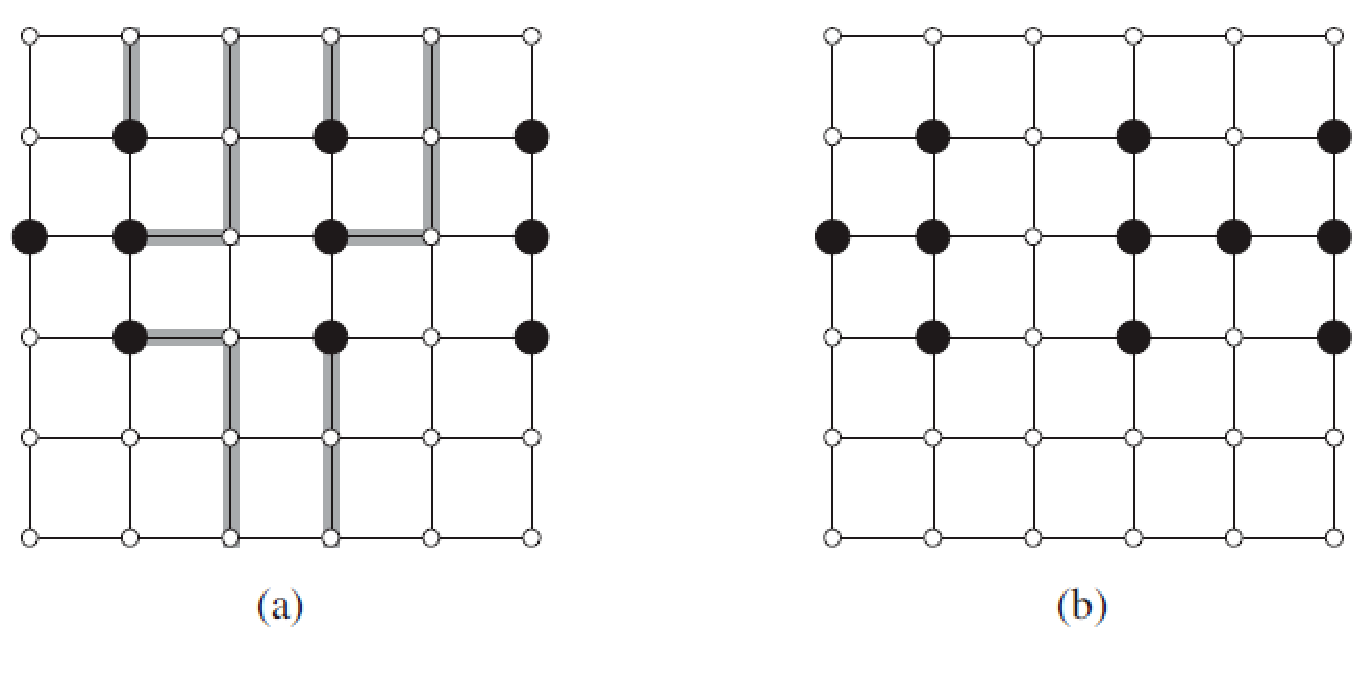
\includegraphics[width=0.5\textwidth]{Fig-EscapeProblem.pdf}
	\caption{Grids for the escape problem. Starting points are black, and other grid vertices are white. (a) A grid with an escape, shown by shaded paths. (b) A grid with no escape.}
	\label{Fig-EscapeProblem}
	\end{figure}
    \begin{enumerate}
        \item Consider a flow network in which vertices, as well as edges, have capacities. That is, the total positive flow entering any given vertex is subject to a capacity constraint. Show that determining the maximum flow in a network with edge and vertex capacities can be reduced to an ordinary maximum-flow problem on a flow network of comparable size. That is, the sizes of the two graph are in the same order of magnitude.
        \begin{solution}
			% 26.1 Max-Flow
			Split the capacity-constraint vertex into two vertices with edges inbetween. The capacity of the edge is the capacity $c$ of the original vertex. And the splited vertices are $v_{in}$ and $v_{out}$, connecting the in-coming edges and out-going edges seperately, shown in Figure \ref{fig:vdir}.

			\begin{figure}[h]
				\centering
				\begin{tikzpicture}
\tikzstyle{ver} = [circle, draw];

\node[ver] (v1) at (0.5,0) {$v$};
\draw (-1,1) edge[->] (v1);
\draw (-1,-1.5) edge [->](v1);
\draw (v1) edge [->](2,1);
\draw (v1) edge [->](2,-1.5);

\node at (3.5,0) {$\Rightarrow$};

\node [ver] (v2) at (6,0) {$v_{in}$};
\node [ver] (v3) at (9,0) {$v_{out}$};
\draw[->]  (v2) edge node[above] {$c$} (v3);
\draw (4.5,1) edge [->](v2);
\draw (4.5,-1.5) edge [->](v2);
\draw (v3) edge [->](10,1);
\draw (v3) edge [->](10,-1.5);
\end{tikzpicture}
				\caption{Vertex split in a directed graph}
				\label{fig:vdir}
			\end{figure}

			As for the undirected graph, the vertices will be splitted any way. But it will be transformed into directed graph by adding more edges, shown in Figure \ref{fig:undir}. The constraint between $v_{in}$ and $v_{out}$ will be the bottleneck even though there are a lot of flow coming into $v_{in}$ and out from $v_{out}$.
			
			% the edge itself will be a bidirectional one with capacity $c$. the flow direction in the edge is depend on the net flow from one splitted vertex to the other, shown in Figure \ref{fig:undir}. In fact, this edge could be  The consevation of flow in and out of vertex tells us that the edges among all of them will be in a equilibrium.

			\begin{figure}[h]
				\centering
				\begin{tikzpicture}
\tikzstyle{ver} = [circle, draw];

\node at (3.5,0) {$\Rightarrow$};

\node [ver] (v1) at (-0.5,0) {$u$};
\node [ver] (v2) at (1.5,0) {$v$};

\draw  (v1) edge node[above] {$w$} (v2);

\node [ver] (v6) at (5,0) {$u_{in}$};
\node [ver] (v3) at (6.5,0) {$u_{out}$};
\node [ver] (v4) at (9,0) {$v_{in}$};
\node [ver] (v5) at (10.5,0) {$v_{out}$};
\draw  (v3) edge[->] node[above] {$w$} (v4);
\draw[out=150,in=30]  (v5) edge[->] node[above] {$w$} (v6);
\draw  (v6) edge[->] node[below] {$c$} (v3);
\draw  (v4) edge[->] node[below] {$c$} (v5);
\end{tikzpicture}

				\caption{Vertex split in an undirected graph}
				\label{fig:undir}
			\end{figure}

			Thus, the vertex magnitude of the reduced graph is $2|V|$, which is the same level as $O(|V|)$. The edge magnitude is at most \begin{tcolorbox}[skin=mycross]
				$2|E|+2|E|$
			\end{tcolorbox}. Because the split on the vertex is only trigged when there is an edge between the two vertices. Then, the edge has the same level as $O(|E|)$.

			% As for the undirected graph, the above method fails to perform. However, because the capacity constraint for every vertex is equal to the same constant. Thus, plug two artifical vertices into the graph to constraint the 
		\end{solution}
        \item Describe an efficient algorithm to solve the escape problem, and analyze its running time.
        \begin{solution}
			The spliting thought could be implemeted in this problem as to plug in two artifical vertices into the graph to constraint the capacity.
			\begin{algorithm}[h]
				\caption{Abstracted Solution to Escape Problem}
				\label{alg:sep}
				Source vertices now share the same source vertex $s$ to get the flow in, shown in Figure \ref{fig:es}\;
				% Split the remaining vertices $v$ except the starting vertices into two vertices\;
				Replace each edge $(u,v)$ in the original graph with edges from $u_{out}$ to $v_{in}$ and from $v_{out}$ to $u_{in}$ of capacity 1, which is similar to Figure \ref{fig:undir}\;
				Target vertices $v_{out}$ now share the same target vertex $v$ to get the flow out\;
				Apply Ford-Fulkerson's algorithm on this problem to find the maximum flow from $s$ to $t$\;
				Determine whether the maximum flow is $m$\;
			\end{algorithm} 
			
			$O(mn^2)$
			
			\begin{tcolorbox}[skin=mycross]
				The time complexity of Algorithm \ref{alg:sep} is $O(2|V|\cdot 4|E|\cdot 1)=O((2n)^2\cdot 4\times 2n(n+1))=O(n^4)$.
			\end{tcolorbox}

			\begin{figure}[h]
				\centering
				\begin{tikzpicture}[node distance=10pt]
\tikzstyle{blackdot} = [circle, fill, scale = 0.5];
\tikzstyle{starter} = [blue!50];
\draw[help lines,line width=1pt]  (-2,2) grid (3,-3);
\node [blackdot] (v3) at (0,1) {};
\node [blackdot] (v2) at (-1,0) {};
\node [blackdot] (v4) at (1,-1) {};
\node [blackdot] (v5) at (2,-2) {};

\node [blackdot,blue] (v1) at (-4,-0.5) {};
\draw [starter] (v1) edge (v2);
\draw [starter] (v3) edge (v1);
\draw [starter] (v4) edge (v1);
\draw [starter] (v5) edge (v1);

\node [blackdot,red] (t) at (5,-0.5) {};
\foreach \x in {-2,-1,...,3}
	\foreach \y in {2,-3}
		\draw[red!50] (\x,\y) edge (t);
\foreach \x in {-2,3}
	\foreach \y in {1,0,...,-2}
		\draw[red!50] (\x,\y) edge (t);

\node [above of=v1,blue] {$s$};
\node [above of=t,red] {$t$};
\end{tikzpicture}
				\caption{With artificial vertices added}
				\label{fig:es}
			\end{figure}

			Firstly, the maximum flow could not exceed $m$ because there are only $m$ edges connecting to $s$. Then, if the maximum flow is less than $m$, then there is no such solution to the original escape problem, because the escape problem requires $m$ total flow.

			If the maximum flow is $m$, then their is a solution to the escape problem. And the solution is the flow except those artifical edges. Because every argumented path will be a unit flow since all the edges share the same constraint of 1. And the capacity constraint on splitted vertices will effect the the edge coming to the vertex. And every flow start from starting point will end up in the border with no vertice on two paths based on the vertex constraint flow network. And that is the solution.
		\end{solution}
    \end{enumerate}
\end{enumerate}

\textbf{Remark:} Please include your .pdf, .tex files for uploading with standard file names.
\newpage


%========================================================================
\end{document}
